\section{Wiener path integral}
The Wiener meosure and the Wiener path integral (Technigiuses and Applications of Both Integration by L.S. Scivemon)
We have seen that the propagator of the Brownion motion satisties the Chapman-Kolunagorov ep. because it is a Markov process.
From ep. (13) and (11)
(14) $w\left(x_{2}, t_{2} \mid x_{0}, t_{0}\right)=\int_{-\infty}^{+\infty} w\left(x_{2}, t_{2} \mid x_{1}, t_{1}\right) w\left(x_{1}, t_{1} \mid x_{0}, t_{0}\right) d x_{1}$

Notice the anology with $Q M:\left\langle x_{2} t_{2} \mid x_{0} t_{0}\right\rangle=w\left(x_{2} t_{2} \mid x_{0} t_{0}\right)$, we insert an identify $\int d x_{1}\left|x_{1}, t_{1}\right\rangle\left\langle x_{1}, t_{1}\right|=1$ and get $\left\langle x_{2} t_{2} \mid x_{0} t_{0}\right\rangle=\int d x_{1}\left\langle x_{2} t_{2} \mid x_{1} t_{1}\right\rangle\left\langle x_{1} t_{1} \mid x_{0} t_{0}\right\rangle$
We con also iterate of (14) $n$-times and get for $t_{n}>t_{m-1}>\ldots>t_{1}>t_{0}$
$w\left(x_{n}, t_{n} \mid x_{0}, t_{0}\right)=\int_{-\infty}^{+\infty} w\left(x_{n}, t_{n} \mid x_{m-1}, t_{m-1}\right) w\left(x_{m-1}, t_{m-1} \mid x_{m-2}, t_{m-2}\right) \ldots$
(14b) ... $\left.w\left(x_{2}, t_{2} \mid x_{1}, t_{1}\right) w\left(x_{1}, t_{1}\right) x_{0}, t_{0}\right) d x_{n-1}, \cdots d x_{1}$

This is an important property of the propagator, because it allows us to understand what is the probability to find a Brownion porticle in different regions at different times. Ondeed, if we define the Wiener measure $t_{m}>t_{m-1}>\ldots>t_{1}>t_{0}$

$$
 d \mathbb{P}_{i, \ldots t_{n}}\left(x_{1} \ldots x_{n} \mid x_{0}, t_{0}\right)=\prod_{1}^{n} w\left(x_{i}, t_{i} \mid x_{i-1}, t_{i-1}\right) d x_{i}
$$

then (intenval $A_{i} \leq \mathbb{R}$ )


\begin{align*}
\mathbb{P}\left(\{A\} \mid x_{0}, t_{1}\right)= & \int_{A_{m}} \int_{A_{m-1}} \cdots \int_{A_{1}} d \mathbb{P}_{t_{1} \cdots t_{n}}\left(x_{1} \cdots x_{n} \mid x_{0}, t_{0}\right)=  \tag{15}\
= & \int_{A_{m}} \int_{A_{m-1}} \cdots \int_{A_{1}} w\left(x_{m} t_{n} \mid x_{m-1} t_{m-1}\right) w\left(x_{m-1} t_{m-1} \mid x_{m-2} t_{m-2}\right) \
& \cdot w\left(x_{1} t_{1} \mid x_{0} t_{0}\right) d x_{m} d x_{m-1} \cdots d x_{1}
\end{align*}

gives the joint probability to find a Brownion porticle in the area $A_{1}$ at time $t_{1}$, within $A_{2}$ at time $t_{2}$ and within $A_{n}$ at time $t_{n}\left(t_{1}<t_{2} \cdots<t_{n}\right)$, given that it started off at $x_{0}$ at time $t_{0}<t_{1}$.
\begin{center}
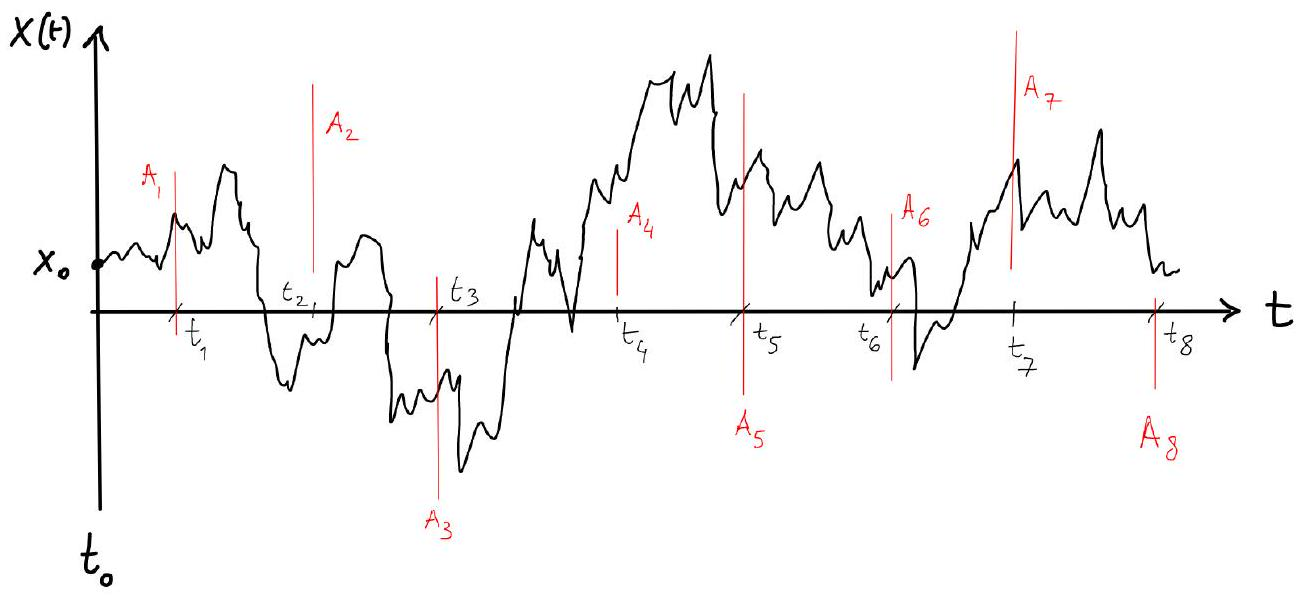
\includegraphics[width=\textwidth]{2025_10_17_55d6813539323d2293f0g-2}
\end{center}

The explicit expression is $\left(\Delta t_{i}=t_{i}-t_{i-1}>0\right)$


\begin{equation*}
d \mathbb{P}_{t_{1} \ldots t_{n}}\left(x_{1} \ldots x_{m} \mid x_{0}, t_{0}\right)=e^{-\frac{1}{2 D} \sum_{i}^{n} i \frac{\left(x_{i}-x_{i-1}\right)^{2}}{\Delta t_{i}}} \prod_{1}^{n} \frac{d x_{i}}{\sqrt{2 \pi D \Delta t_{i}}} \tag{16}
\end{equation*}


This relation is valid for any $n \in \mathbb{N}$ and we con extend the vesult to any subset of the 6 -algebra generated by the cylindrical sets of the form $A=\left\{x(t): x\left(t_{1}\right) \in A_{1}, x\left(t_{2}\right) \in A_{2} \ldots x\left(\mathrm{t}_{n}\right) \in A_{n}\right\}$. When we take the limit $n \rightarrow \infty$ we obtain the $\infty$ called Wiener path integral. On this case

$$ 
\sum_{i}^{n} \frac{\left(x_{i}-x_{i-1}\right)^{2}}{\Delta t_{i}}=\sum_{1}^{n} i\left(\frac{x_{i}-x_{i-1}}{\Delta t_{i}}\right)^{2} \Delta t_{i} \xrightarrow[\sum_{i} \Delta t_{i}=T]{m \overrightarrow{\operatorname{mox}}\left(\Delta t_{i}\right) \rightarrow 0} \int_{0}^{T}(\dot{x}(s))^{2} d s
$$ 

and ey. (16) gets the suggestive form


\begin{equation*}
d \mathbb{P}_{w}=r \prod_{r=0^{+}}^{T} e^{-\frac{1}{2 D} \int_{0}^{T} \dot{x}(s)^{2} d s} d x(r) \tag{17}
\end{equation*}


This formula is only formal as it does not exist (it is infinite!). However, it is very useful for colculating averages of functionals which are
exponentials of quodratic expressions of the trajectory $x(s)$ or for approximations with the saddle point method.
Another way to look at ey. (146) is the following. We fix $x_{n}=x$, $t_{n}=T$ and $x_{0}$ at $t_{0}$. Then all the integrations $x_{n-1}, x_{n-2} \ldots, x_{1}$ at the corrisponding ordered times $t_{m-1}, \ldots t_{1}$ show that in the limit $n \rightarrow \infty$ (with fixed $x, T ; x_{0}, t_{0}$ ) the propagator of a Brownion porticle $W\left(x_{1} T \mid x_{0}, t_{0}\right)$ con be written as
$w\left(x, T \mid x_{0}, t_{0}\right)=\int_{x(0)=0}^{x(T)=x} D x(r) e^{-\frac{1}{2 D} \int_{0}^{T} \dot{x}(s)^{2} d s}=\int_{x(0)=0}^{x(T)=x} D x(r) e^{-s[x(s)]}$
(17b)
\begin{center}
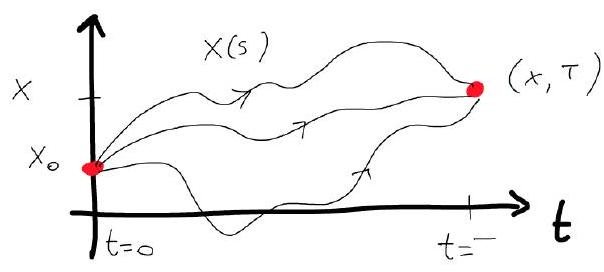
\includegraphics[width=\textwidth]{2025_10_17_55d6813539323d2293f0g-3}
\end{center}
the propogetor $W$ con be written as an integral over all trajectories between ( $0, x_{0}$ ) and ( $\tau, x$ ) of the Brownion perticle.

Here $S[x(s)]$ is the action and $S=\int_{0}^{T} L[x] d s$, where $L$ is the Logrongion of the system. Here $L[x(s)]=\frac{1}{2 D}\left(\frac{d x}{d s}\right)^{2}$ which can be interpreted as the kinctic energy of a free particle. Furthermone, notice that if we change variable $s=i t / \hbar$ (as an analytic continuation), identify $D=\frac{\hbar^{2}}{m}$ and introduce the "imoginary" time $\tilde{t}=-i \hbar T$, then the propogetor in (17b) becomes
$W\left(x, \tilde{t} \mid x_{0}, 0\right)=\int_{x(0)=0}^{x(\tilde{t})=x} D x\left(z^{\prime}\right) e^{\frac{i}{\hbar} \int_{0}^{\tilde{t}} \frac{1}{2} m\left(\frac{d x}{d t^{\prime}}\right)^{2} d t^{\prime}}=\sqrt{\frac{m}{2 \pi \hbar \tilde{t}}} e^{\frac{i m}{2 \hbar \tilde{t}}\left(x-x_{0}\right)^{2}}$
(17.c) $\int_{\text {using ey. (13) with } x_{1}=x_{i} t_{1}=T}^{t_{0}=0}$
This is the propogator (or Green's function) of the Schrödinger es:

$$ 
i 
 i \hbar \frac{\partial \psi}{\partial E}=\hat{H} \psi \quad \text { where } \quad \hat{H}=-\frac{\hbar^{2}}{2 m} \frac{\partial^{2}}{\partial x^{2}}
$$ 

we con write $W\left(x, \tilde{E} \mid x_{0}, 0\right)=\langle x| e^{-\frac{i}{\hbar} \tilde{E} \hat{H}}\left|x_{0}\right\rangle$
and conespondingly we can also write $\hat{H}|k\rangle=\frac{\hbar^{2}}{2 m} k^{2}|k\rangle=\frac{D k^{2}}{2}|k\rangle$

$$ 
\begin{aligned}
W\left(x, T \mid x_{0}, 0\right) & =\langle x| e^{-T H}\left|x_{0}\right\rangle=\int d k \int d k^{\prime}\left\langle x \mid k^{\prime}\right\rangle\left\langle k^{\prime}\right| e^{-T H}|k\rangle\langle k \mid x\rangle=\\
= & \frac{1}{2 \pi} \int d k e^{-\frac{D}{2} T k^{2}} e^{i k\left(x-x_{0}\right)}=\frac{1}{\sqrt{2 \pi D T}} e^{-\frac{\left(x-x_{0}\right)^{2}}{2 D T}} \quad\left\langle x \mid k^{\prime}\right\rangle=\frac{1}{\sqrt{2 \pi}} e^{i k^{\prime} x}
\end{aligned}
$$ 

This con be generalized to the cose of $\hat{H}=-\frac{\hbar^{2}}{2 m} \frac{\partial^{2}}{\partial x^{2}}+V(x)$ (Schuluman, (h.g)) Similar connections to statistical rechamics as $T \rightarrow \beta(c h, 26)$.

\section*{Two-point covelation function (exercize)}
With the help of e. (16) it is casy to colculate the 2 -point correlation function which is defined as $\left\langle x\left(t_{1}\right) x\left(t_{2}\right)\right\rangle$ for $t_{0}<t_{1}<t_{2}$. We assume that the particle starts at $x_{0}=x\left(t_{0}\right)$.
\begin{center}
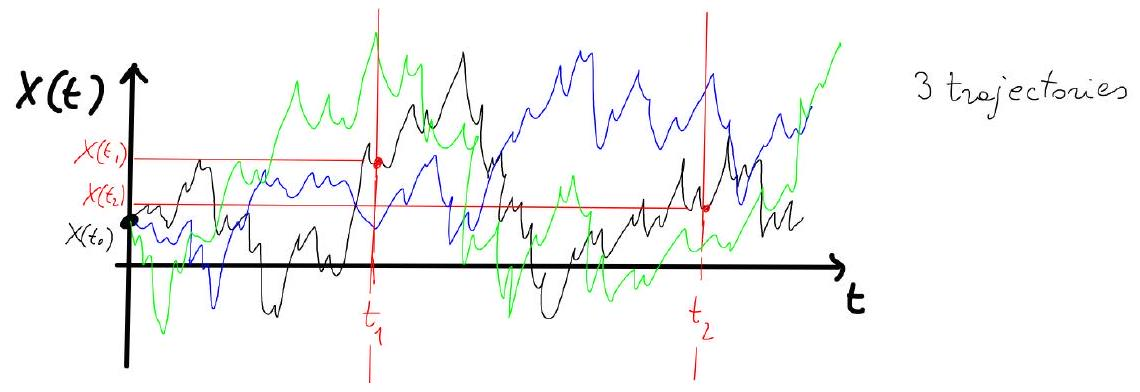
\includegraphics[width=\textwidth]{2025_10_17_55d6813539323d2293f0g-4}
\end{center}

A verge over Brownion hajectories, all starting at $x_{0}$ at time $t=t_{0}$, when looking at the trajectories at times $t=t_{1}$ and $t=t_{2}$.


\begin{align*}
& \left\langle x\left(t_{1}\right) x\left(t_{2}\right)\right\rangle_{w}=\iint d \mathbb{P}_{t_{1} t_{2}}\left(x_{1}, x_{2} \mid x_{0}, t_{0}\right) x_{1} x_{2}  \tag{18}
\\
& =\int_{-\infty}^{+\infty} d x_{2} \int_{-\infty}^{+\infty} d x_{1} \frac{1}{\sqrt{2 \pi D\left(t_{2}-t_{1}\right)}} e^{-\frac{1}{2 D} \frac{\left(x_{2}-x_{1}\right)^{2}}{t_{2}-t_{1}}} \frac{1}{\sqrt{2 \pi D\left(t_{1}-t_{0}\right)}} e^{-\frac{1}{2 D} \frac{\left(x_{1}-x_{0}\right)^{2}}{t_{1}-t_{0}}} x_{2} x_{1}
\end{align*}


We change veriables: $x=x_{1}-x_{0}, y=x_{2}-x_{1}$

$$ 
 x_{2}=x_{0}+x+y \quad x_{1}=x+x_{0} \quad\left(x_{0} \text { is a const. }\right)
$$ 

Remember the Jacobian in the trousformation:

$$ 
\begin{array}{r}
p\left(x_{1}, x_{2}\right) d x_{1} d x_{2}=p\left(x_{1}(x, y), x_{2}(x, y)\right)|J| d x d y \
J=\left(\begin{array}{cc}
\frac{\partial x_{1}}{\partial x} & \frac{\partial x_{1}}{\partial y} \\ 
\frac{\partial x_{2}}{\partial x} & \frac{\partial x_{2}}{\partial y}\end{array}\right)=\left(\begin{array}{cc}1 & 0 \\ 1 & 1\end{array}\right) \Rightarrow|J|=1
\end{array}
$$ 

From op. (18) we get

$$ 
\begin{aligned}
& =\int_{-\infty}^{+\infty} d x \int_{-\infty}^{+\infty} d y \frac{1}{\sqrt{2 \pi D\left(t_{2}-t_{1}\right)}} e^{-\frac{1}{2 D} \frac{y^{2}}{t_{2}-t_{1}}} \underbrace{e^{-\frac{1}{2 D} \frac{x^{2}}{t_{1}-t_{0}}}\\left(x_{0}+x+y\right)\\left(x+x_{0}\right)}_{\begin{array}{c}\n\left\langle x^{2}\right\rangle \neq 0 \\ x^{2}+\underbrace{x_{0}(2 x+y)+x y}_{\langle x\rangle=\langle y\rangle=0}+x_{0}^{2} \\ \frac{1}{2 \pi D\left(t_{1}-t_{0}\right)}
\end{array}}
\\ 
& =\int_{-\infty}^{+\infty} d x \frac{e^{-\frac{x^{2}}{2 \Delta\left(t_{1}-t_{0}\right)}}}{\sqrt{2 \pi D\left(t_{1}-t_{0}\right)}} x^{2}+x_{0}^{2} \\
& =D\left(t_{1}-t_{0}\right)+x_{0}^{2} \quad \int_{-\infty}^{+\infty} x^{n} e^{-\frac{a x^{2}}{2}} d x=\frac{(n-1)(n-3) \cdots 5 \cdot 3 \cdot 1 \sqrt{2 \pi}}{a^{(n+1) / 2}} \\
& t_{2}>t_{1}>t_{0}
\end{aligned}
$$ 

Thus for a generic poir of times $t_{1}, t_{2}>t_{0}$:
(19) $\left\langle x\left(t_{1}\right) x\left(t_{2}\right)\right\rangle_{w}=D \min \left\{t_{1}, t_{2}\right\}+x_{0}^{2}$

Exercize: colculate $\left\langle x\left(t_{1}\right) x\left(t_{2}\right)\right\rangle_{w}$ for a generic imitial distribution $g\left(x_{0}\right)$.

Averaging a functional with the Wiener path integral.
Functionals of trajectories (say, porition of a particle in time) occur many times in Physics. For example, one may wont to colculate the average of $F\left(\int_{0}^{T} a(s) x(s) d s\right)$, where $x(s)$ is the volve of the Brownion trajectory at time $s$, $a(s)$ is a smooth function of time and $F$ is another runoth function.

For any specific colulation we will sely on the discrete, finite $x$, formula in eg. (16). Namely, if we wish to find the expected value of a functional such as $F\left(\int_{0}^{T} a(t) x(t) d t\right)$, we finst take its discrite version, $\sum_{i}{a} \Delta t_{i} a\left(t_{i}\right) \times\left(t_{i}\right)$, use ep. (16) for the colculations and only at the end we take the limit $n \rightarrow \infty, \Delta t \rightarrow 0$.

In the following we will also use the function $A(s)=\int_{s}^{T} a(\tau) d \tau$ which satisfies $\dot{A}(S)=-a(S)$ and $A(T)=0$. Now, $x(0)=0 \left.\int_{0}^{T} a(s) x(s) d s=-\left.x(s) \int_{s}^{T} a(\tau) d \tau\right|_{s=0} ^{s=T}+\int_{0}^{T} \dot{x}(s) \int_{s}^{T} a(\tau) d \tau\right) d s=\int_{0}^{T} \dot{x}(s) A(s) d s$

This can be written down in the discrete form as

$$ 
\int_{0}^{T} A(s) \dot{x}(s) d s=\int_{0}^{x(T)} A(S(x)) d x=\lim _{\substack{n \rightarrow \infty \\ \max _{i}\left(\Delta x_{i}\right) \rightarrow 0}} \sum_{1}^{n} A_{i} \underbrace{x_{i}-x_{i-1}}_{\equiv \Delta x_{i}})
$$ 

From now on we set $2 D=1$ (in the end we replace $t \rightarrow 2 D t$ ) We use the Wiener measure in ep. (16) and calculate the overage of the discretized functional $F,\left\langle I_{n}\right\rangle$, for a fixed $n$ :\n(20) $\left\langle I_{n}\right\rangle=\int_{\mathbb{R}^{n}} \pi_{i}^{n} \frac{d x_{i}}{\sqrt{\pi \Delta t_{i}}} F\left(\sum_{i}^{n} A_{i} \Delta x_{i}\right) e^{-\sum_{i}^{n} \cdot \frac{\left(\Delta x_{i}\right)^{2}}{\Delta t_{i}}}$

Now we change variables: $y_{i}=\Delta x_{i}$, so $x_{i}=\sum_{p}^{i} y_{k}+x_{0}$ for $i=1,2 \ldots, n$
Remember: $\quad q(\{y\})=p(\{x(y)\})\left|\frac{\partial x}{\partial y}\right|$

We have to be coreful about the jacobian $J$ :\n$J=\left(\begin{array}{cccc}\frac{\partial x_{1}}{\partial y_{1}} & \frac{\partial x_{1}}{\partial y_{2}} & \cdots & \frac{\partial x_{1}}{\partial y_{m}} \\ & \cdots & & \\ \frac{\partial x_{m}}{\partial y_{1}} & \frac{\partial x_{m}}{\partial y_{2}} & \cdots & \frac{\partial x_{m}}{\partial y_{m}}\end{array}\right)=\left(\begin{array}{cccc}1 & 0 & \cdots & 0 \\ 1 & 1 & \cdots & 0 \\ 1 & \cdots & & \vdots \\ \vdots & 1 & \cdots & 1 \\ 1 & 1 & \cdots & 1\end{array}\right) \Rightarrow \operatorname{det} J=1$
hhence
(21) $\left\langle I_{n}\right\rangle=\int_{\mathbb{R}^{n}} \prod_{i}^{n} \frac{d y_{i}}{\sqrt{\pi \Delta t_{i}}} F\left(\Sigma_{i} A_{i} y_{i}\right) e^{-\frac{\Sigma_{i} y_{i}^{2}}{\Delta t_{i}}}$

Now we use a little trick. As $\delta(z)=\frac{1}{2 \pi} \int_{-\infty}^{+\infty} e^{i x z} d x$ and $F\left(\Sigma_{i} A_{i} y_{i}\right)=\int F(z) \delta\left(z-\Sigma_{i} A_{i} y_{i}\right) d z$, we con write ep. (21) as

$$ 
\begin{aligned}
& \left\langle I_{n}\right\rangle=\int \pi_{i} \frac{d y_{i}}{\sqrt{\pi \Delta t_{i}}} \int \frac{d x}{2 \pi} d z F(z) e^{i x\left(z-\sum_{j} A_{j} y_{j}\right)} e^{-\frac{\sum_{i} y_{i}^{2}}{\Delta t_{i}}} \\ 
& =\int_{-\infty}^{+\infty} \frac{d x d z}{2 \pi} e^{i x z} F(z) \int_{\mathbb{R}^{n}} \pi_{i} \frac{d y_{i}}{\sqrt{\pi \Delta t}} e^{-\sum j\left(\frac{y_{j}^{2}}{\Delta t_{j}}+i A_{j} y_{j} x\right)} \\ 
& \text { Gaussion } \\
& \text { integrals! } \\
& =\int_{-\infty}^{+\infty} \frac{d x d z}{2 \pi} e^{i x z} F(z) e^{-\frac{x^{2}}{4} \sum_{i} A_{i}^{2} \Delta t_{i}}=\int d z F(z) \int \frac{d x}{2 \pi} e^{-\frac{x^{2}}{4} \sum_{i} A_{i}^{2} \Delta t_{i}+i x z} \\ 
& =\int d z F(z) \frac{e^{-\frac{z^{2}}{\sum_{i} A_{i}^{2} \Delta t_{i}}}}{\left(\pi \sum_{i} A_{i}^{2} \Delta t_{i}\right)^{1 / 2}}=\int_{-\infty}^{+\infty} d z F(z) N_{z}\left(0, \Sigma_{i} A_{i}^{2} \Delta t_{j}\right)
\end{aligned}
$$ 

Hence
(22) $\left\langle I_{1}\right\rangle=\left\langle F\left(\hat{\sum}_{i} A_{i} \Delta x_{i}\right)\right\rangle_{B M}=\int_{-\infty}^{+\infty} d z F(z) N_{z}\left(0, \varepsilon_{i} A_{i}^{2} \Delta t_{i}\right)$

Where $N_{z}\left(\mu, \sigma^{2}\right)$ is the Normal distribution with mean $\mu$ and variance $\sigma^{2}$. We can now take the limit $n \rightarrow \infty, \Delta t ; \rightarrow 0$ :\n(23) $\quad \sum_{i} A_{i}^{2} \Delta t_{i} \longrightarrow \int_{0}^{T} A^{2}(s) d s=\int_{0}^{T}\left(\int_{s}^{T} a(z) d z\right)^{2} d s \equiv R(T)$

Thus the continuum formulation gives:
(24) $\left\langle F\left(\int_{0}^{T} a(s) x(s) d s\right)\right\rangle_{B M}=\int_{-\infty}^{+\infty} d z F(z) N_{z}(0, R(T))$
where $R(T)$ is defined in (23). If we introduce $2 D$, we get

$$ 
N_{z}(0, R(T))=\frac{1}{\sqrt{2 \pi D R(T)}} e^{-\frac{z^{2}}{2 D R(T)}}
$$ 

Example:
If $F(z)=e^{h z}$ we obtain the moment generating function of $\int_{0}^{T} a(s) x(s) d s$, namely

$$ 
\left\langle e^{h \int_{0}^{T} Q(s) \times(s) d s}\right\rangle_{BM}=e^{\frac{D R(T)}{2} h^{2}}
$$ 

Exercige: Take $F(z)=e^{z}, a(s)=h_{1} \delta\left(t_{1}-s\right)+h_{2} \delta\left(t_{2}-s\right)$ for $0<t_{1}, t_{2}<T$. Calculate $A(s)$ and $R(T)$. Since $\int_{0}^{T} a(s) x(s) d s=h_{1} x\left(t_{1}\right)+h_{2} x\left(t_{2}\right)$, calculate $z\left(h_{1}, h_{2}\right)=\left\langle e^{h_{1} x\left(t_{1}\right)+h_{2} x\left(t_{2}\right)}\right\rangle_{w}$ and finally show that


\begin{equation*}
\left.\frac{\partial^{2} z}{\partial h_{1} \partial h_{2}}\right|_{h_{1}=\theta=h_{2}}=\left\langle x\left(t_{1}\right) x\left(t_{2}\right)\right\rangle_{BM}=D \min \left\{t_{1}, t_{2}\right\} \tag{19}
\end{equation*}


\section*{A brief summary of what we have done:}
We have learnt some properties of the Browmion process:

\begin{enumerate}
  \item It is the most important continuous stochostic process, which is tightly linked to the diffusion equation. It is a Markov process with continuous paths, but very irregular ones as it is nowhere differentiable.
  \item We know how to simulate it.
  \item It con be used to define a poth integral, an object that is not very well defined but (at least in its discrete form) it con be used to colulate some functionals thot are useful in Physics and beyoud.
\end{enumerate}

At this point we want to use the Brownion motion to build up new continuous stochastic processes. We will do that by defining stochastic differential apuations (SDEs). This needs a lot of core because there are many subleties with continuous stochastic processes. We will look into the main feotures. There are many books which develop SDES rigorously.